\documentclass{article}


% if you need to pass options to natbib, use, e.g.:
%     \PassOptionsToPackage{numbers, compress}{natbib}
% before loading neurips_2022

% References (added by Sophia)
% https://www.overleaf.com/learn/latex/Bibliography_management_in_LaTeX
% https://en.wikibooks.org/wiki/LaTeX/Bibliography_Management
\usepackage[authordate,bibencoding=auto,strict,backend=biber,natbib]{biblatex-chicago}
\usepackage[english]{babel}
\addbibresource{References.bib}

\DefineBibliographyStrings{english}{%
  andothers = {et al.},
}

\usepackage[pdftex]{graphicx}

% ready for submission
\usepackage[final,nonatbib]{neurips_2022}


% to compile a preprint version, e.g., for submission to arXiv, add add the
% [preprint] option:
%     \usepackage[preprint]{neurips_2022}


% to compile a camera-ready version, add the [final] option, e.g.:
%     \usepackage[final]{neurips_2022}


% to avoid loading the natbib package, add option nonatbib:
%    \usepackage[nonatbib]{neurips_2022}


\usepackage[utf8]{inputenc} % allow utf-8 input
\usepackage[T1]{fontenc}    % use 8-bit T1 fonts
\usepackage{hyperref}       % hyperlinks
\usepackage{url}            % simple URL typesetting
\usepackage{booktabs}       % professional-quality tables
\usepackage{amsfonts}       % blackboard math symbols
\usepackage{nicefrac}       % compact symbols for 1/2, etc.
\usepackage{microtype}      % microtypography
\usepackage{xcolor}         % colors



\title{From healthy to diseased; using scVI to detect nonlinear gene expression changes on paths between healthy and sick cells in latent space}


% The \author macro works with any number of authors. There are two commands
% used to separate the names and addresses of multiple authors: \And and \AND.
%
% Using \And between authors leaves it to LaTeX to determine where to break the
% lines. Using \AND forces a line break at that point. So, if LaTeX puts 3 of 4
% authors names on the first line, and the last on the second line, try using
% \AND instead of \And before the third author name.


\author{%
Yegor Kuznetsov$^{1}$ \quad Sophia Jannetty$^{2}$\\
$^1$University of Washington Department of Computer Science\\
$^2$University of Washington Department of Biology\\
\texttt{yegor@uw.edu}\\
\texttt{jannetty@uw.edu}\\
}


\begin{document}


\maketitle


\begin{abstract}
  Researcers comparing sick cell transcription profiles to healthy cell transcription profiles may miss important information about intermediate transitioning transcription profiles not represented in healthy or sick datasets.
  Without time-series data calibrated to degree of disease progression, analyzing changes in transcriptional profiles as diseases progress over time can be challenging.
  Here we investigate the possibility of generating and analyzing artificial transcription data for cells transitioning from a healthy to a sick state.
  Using the deep generative modeling technique scVI \citep{lopez_deep_2018}, we embed published scRNAseq data from sick and healty cells into a learned 10-dimensional latent space.
  We then sample the latent space on paths between sick and healthy cells in latent space and use the model decoder to generate transcriptional profiles for cells that would exist at each location.
  We then analyze these transcriptomes and identify genes that have a nonlinear predicted trajectory on the path between healthy and sick.
  We propose future methods for investigating and validating this method.
\end{abstract}


\section{Introduction}

Differential expression analysis is a common technique for assessing differences between transcriptional profiles of healthy and sick cells\citep{anders_differential_2010}.
However, differential expression analysis may miss transient changes in expression that occur as a cell transitions from healthy to sick (Figure \ref*{motivation}).
We aim to develop a technique that builds on recent advances in scRNAseq analysis to address this limitation.

Several recent papers have demonstrated how neural networks can be used to embed scRNA-seq data in low-dimensional latent space \citep{ding_interpretable_2018,wang_vasc_2018,gronbech_scvae_2018,eraslan_single-cell_2019}.
Emphasized utilities of these methods have included effective denoising \citep{eraslan_single-cell_2019}, dimensionality reduction \citep{wang_vasc_2018,ding_interpretable_2018}, and visualization \citep{wang_vasc_2018}.
Several of these methods also provide decoders that allow for translation from latent space back into gene space.
\citet{gronbech_scvae_2018} and \citet{lopez_deep_2018} both discuss decoding latent-space representations of cells by using a nonlinear decoder to generate a posterior estimate of the expression of each gene in a cell.
Our project is focused on investigating the possibility of using these tools to learn about changes in gene expression patterns as a cell transitions from healthy to sick.

Throughout this project we aim to explore the following enormous assumption; given a latent space in which healthy and sick cells cluster apart from each other (such that there are healthy regions and sick regions in the space), do decoded locations between these regions correspond to transcriptional profiles of cells in transition between healthy and sick?
Furthermore, do decoded locations closer to healthy regions than to sick regions correspond to transcriptional profiles of cells that are only slightly sick (and vice versa)?
We begin by operating as though this is a fair assumption.
We tried using this method using two separate datasets (both relevant to hematopoietic stem and progenitor cells, or HSPCs).
For each, we trained the scVI model on scRNA-seq data with sick and healthy labels.
Once scVI embedded each cell in latent space, we sampled the space between healthy and sick cells and used the model's nonlinear decoder to generate transcriptional profiles corresponding to each location.
We then analyzed the model-predicted changes in gene expressions.
Figure \ref*{approach} gives a broad overview of our approach.

\begin{figure}
  \centering
  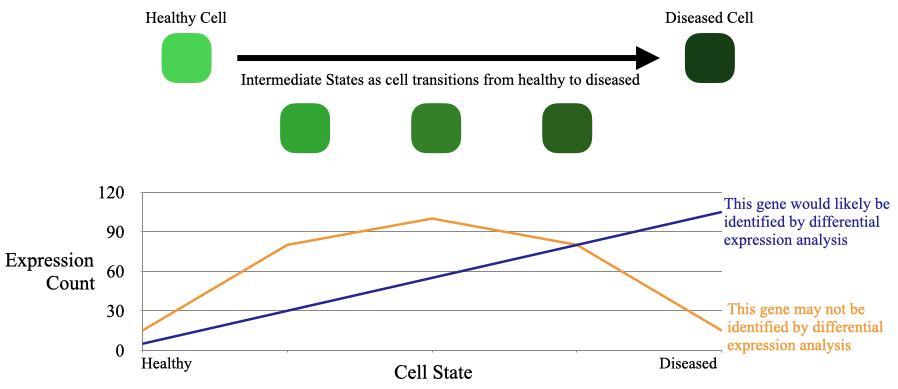
\includegraphics[width=0.9\textwidth]{cropped_motivation.jpg}
  \caption{Project motivation.
  Differential expression analysis is effective at identifying genes that have different rates of transcription between healthy and sick cells.
  However, differential expression analysis may not identify genes that have transient changes in expression as cells transition from healthy to sick.}
  \label{motivation}
\end{figure}

\subsection{Related Work}
Our method heavily builds upon pseudotime.
Pseudotime \citep{reid_pseudotime_2016} is a method for estimating a cell's progress through a given transition.
Pseudotime takes transcriptional data (scRNAseq data or microarray data) from cells assumed to be at various phases of a given transition.
The method then embeds this data in a latent space with an enforced structure related to the temporal capture time of each cell \citep{reid_pseudotime_2016}.
The resulting latent dimension corresponds to pseudotime.
Using this method, researchers can take a set of transcriptional profiles and order them by their phase in progression between one state and another.
However, this method is both supervised (in that it imposes a time-related restraint on its latent space) and is only effective on datasets in which cells are at various stages of progression.
This method cannot be used to generate predicted transcriptional profiles of cells at a certain phase of transition if cells in that phase of transition do not exist in the dataset.

Our method is also related to pathway analysis methods like TIPS \citep{zheng_tips_2021} and MetaCell \citep{baran_metacell_2019}.
TIPS orders cells in pseudotime and then uses prior knowledge of the data to investigate changes in specific, hypothetically relevant genes' expressions as cells progress through pseudotime \citep{zheng_tips_2021}.
This method is an exciting progression of pseudotime, however it also can only draw observations about changes in gene expression levels captured within the dataset.
Additionally, TIPS relies on prior knowledge to identify genes to investigate.
MetaCell generates composite cell profiles from cells that cluster by similarity to minimize noise, allowing for analysis between different cell types.
This method also has a supervised component (in that the genes used to calculate similarity between cells are selected by the researcher) and does not ensure that cells at different phases in a transition will be represented in seperate composite profiles.

Our work is, to our knowledge, unique in two ways.
First, our method aims to identify transcriptional changes over transitional phases without assuming cells of each phase are represented in the dataset.
We are assuming we have a starting point and an ending point, and are generating transcriptional profiles for intermediate transitional phases sampling the latent space between these starting and ending points.
Second, our method is entirely unsupervised.
We aim to detect genes that undergo transcriptional changes over a transition with no prior knowledge of the cells or the transition in place.

% The scVI method described in \citet{lopez_deep_2018} is unique from previous methods due to its explicit consideration of library size and batch effects.
% \citet{lopez_deep_2018} demonstrated that their model could be used to perform batch removal, normalization, dimensionality reduction, clustering, and differential expression analysis.
\subsection{Datasets}
For this project, we worked with two different datasets; an Aplastic Anemia dataset published by \citet{tonglin_single-cell_2022}, and a Chronic Myelomonocytic Leukemia dataset published by \citet{ferrall-fairbanks_progenitor_2022}.

\begin{figure}
  \centering
  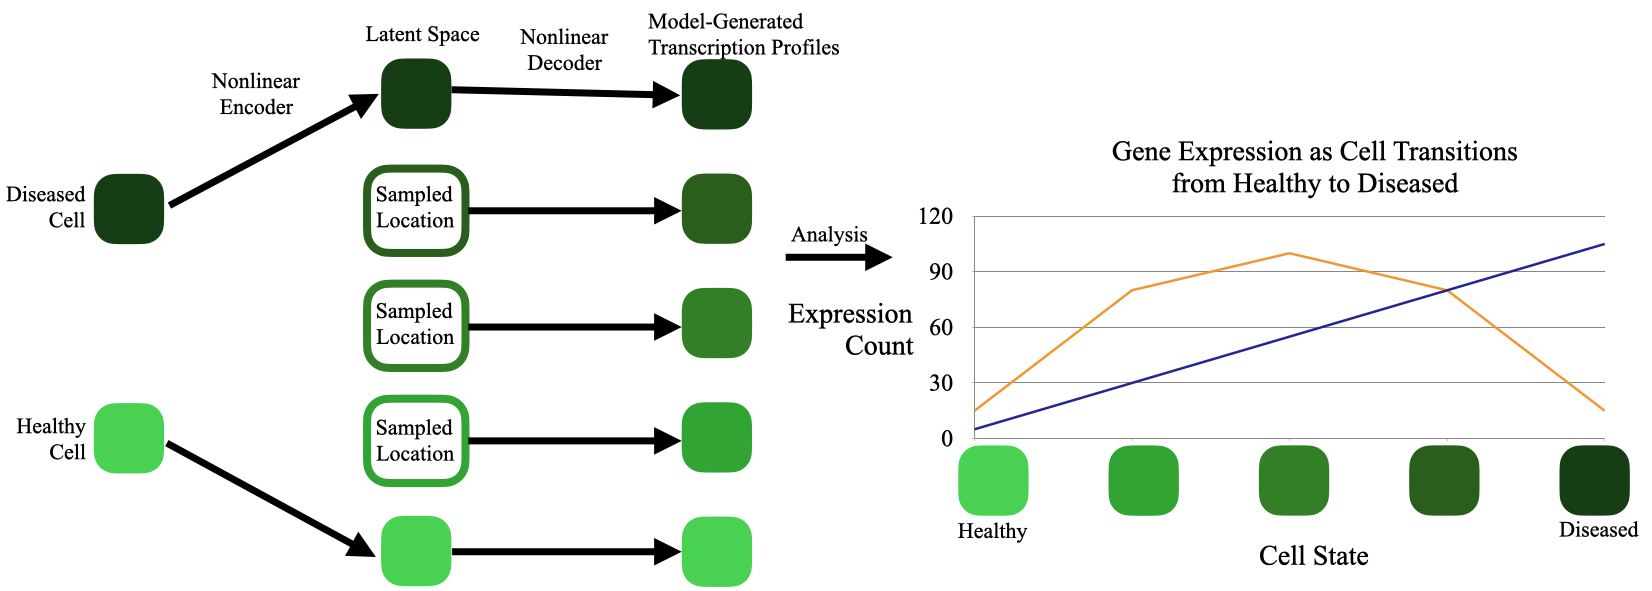
\includegraphics[width=0.9\textwidth]{cropped_approach.jpg}
  \caption{A schematic of our approach. 
  We trained scVI on scRNA-seq data of healthy and diseased cells.
  We then sampled locations on the lines between healthy and diseased cells in latent space and used scVI's decoder to generate transcriptional profiles from these sampled locations.
  We then analyzed the changes in expression of each gene over time.}
  \label{approach}
\end{figure}


\begin{figure}
  \centering
  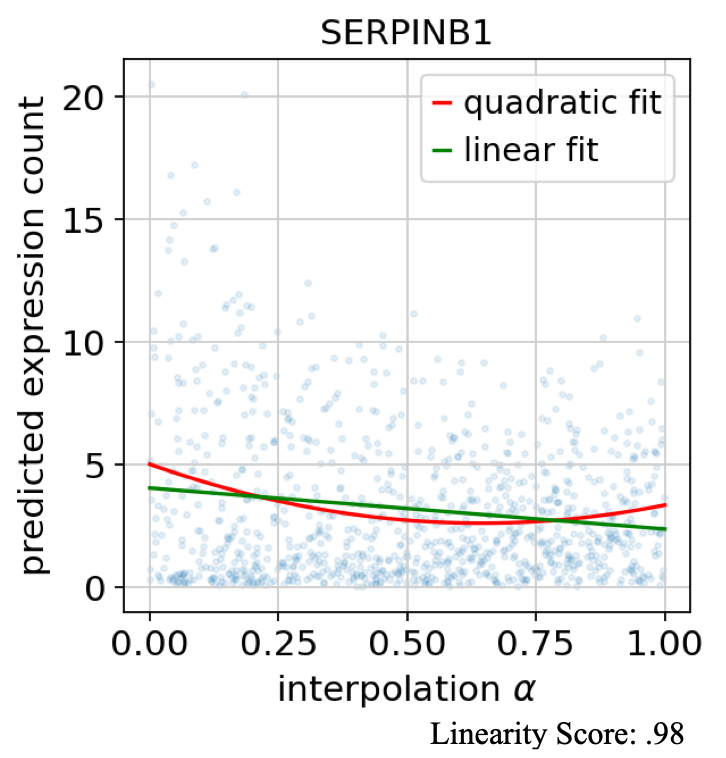
\includegraphics[width=0.5\textwidth]{SERPINB1.jpg}
  \caption{An example of a highly ranked gene in our analysis generated from the \citet{ferrall-fairbanks_progenitor_2022} Leukemia data.
  SERPINB1 is a neutrophil serine protease inhibitor that protects the cell from proteases released in the cytoplasm during stress or infection.}
  \label{SERPINB1_graph}
\end{figure}

\subsubsection{Aplastic Anemia}
Aplastic anemia (AA) is a condition in which a patient\textquotesingle s bone marrow fails to form enough red blood cells, white blood cells, and platelets, resulting in pancytopenia \citep{young_aplastic_2018}.
Pathophysiological mechanisms of this disease include direct damage to bone marrow (commonly from chemotherapy), germ line loss-of-function mutations that interfere with blood-cell precursor DNA repair pathways, and autoimmune attack \citep{young_aplastic_2018}. 

% Current options for treating AA fall within three categories, each of which attempts to address pancytopenia in a different way.
% The first, bone marrow transplantation, aims to replace failing bone marrow with healthy donor marrow. 
% This is a curative treatment, but is limited by the prevalence of graft-versus-host disease and by its reliance on tissue donors \citep{young_aplastic_2018}.
% Furthermore, the survival rate for adults over the age of 40 following bone marrow transplantation is only around 50\% \citep{giammarco_transplant_2018}.
% The second, immunosuppression, aims to eliminate immune-mediated AA.
% This category includes treatment with antilymphocyte globulin (combined with cyclosporine), which has a mild lymphocyte-depleting effect.
% This treatment leads to improved blood production in about 66\% of patients \citep{bacigalupo_how_2017}, however 30\% to 60\% of these patients experience relapse that requires years of continued cyclosporine therapy \citep{scheinberg_activity_2012}.
% Despite the success of immunosuppressant treatments, the mechanisms by which the immune system damages bone marrow remain unknown; the strongest evidence for immune-mediation of aplastic anemia is the effectiveness of immunosuppressant treatments \citep{young_aplastic_2018}.
% The third treatment category, stem-cell stimulation, aims to promote stem-cell regeneration within the patient directly.
% One such treatment involves administrating eltrombopag, a synthetic mimic of thrombopoietin (a hormone that stimulates the production of platelets).
% This treatment has been shown in limited clinical trials to improve blood production in 80\% of treated patients, though the mechanism of this treatment remains unknown \citep{young_aplastic_2018}.

Despite the severity of this disease, the mechanisms underlying its onset remain obscure due to limitations in experimental techniques.
It is thought that T cells may target hematopoietic stem and progenitor cells (HSPCs), which are blood cell precursor cells, in patients with immune-mediated AA \citep{tonglin_single-cell_2022}.
Understanding the transcriptional differences an HSPCs undergoes as it progresses from healthy to AA could uncover the cause of the T cell targeting.
However HSPCs are severely depleated in AA patients, making them a difficult target to study \citep{zhu_single-cell_2021}.
Recent studies like \citet{tonglin_single-cell_2022} and \citet{zhu_single-cell_2021} have used single-cell RNA-sequencing (scRNA-seq) to perform differential expression analysis between healthy and AA patient HSPCs.
% These studies have thus far used PCA to reduce dataset dimensionality, followed by graph-based clustering and likelihood ratio tests to identify significantly differentially expressed genes between clusters \citep{zhu_single-cell_2021}.
% These studies have successfully identified differentially expressed genes between healthy and AA HSPCs.
% However, their adjustments for noise and batch effects are limited to their initial dimension reductions.
% This initial dimension reduction assumes a generalized linear model is sufficient for accurately mapping onto the low-dimensional manifold underlying the data.
% This is a particularly problematic assumption in papers like \citet{tonglin_single-cell_2022} where samples were only taken from four patients (two healthy and two with AA).
% With such a low n of patients, it would be challenging to convincingly claim differences between AA and healthy clusters are due to disease status as opposed to being due to differences between individuals.
However, these analyses will only identify genes that have different expression levels between sick and healthy cells.
We aim to identify potential transient changes in gene expression that characterize an HSPC's transition from healthy to AA.

% In this project we explored methods of learning differences between healthy and AA HSPCs using the scRNA-seq data published by \citet{tonglin_single-cell_2022}.
% We used computational methods to model both healthy and diseased HSPC transcriptome profiles with the goal of identifying perturbations capable of moving a diseased HSPC to a healthy cell or vice versa.
% Such identified perturbations could both suggest potential new therapies and help identify the mechanisms of AA onset and treatment.
% We have not yet reached this goal of identifying perturbations.
% However, our work sheds light on what methods are useful when working with data collected from a very small number of individuals.

\subsubsection{Chronic Myelomonocytic Leukemia}
Chronic Myelomonocytic Leukemia is a cancer of the blood in which patient bone marrow makes too many white blood cells (monocytes) \citep{ferrall-fairbanks_progenitor_2022}.
We selected the Chronic Myelomonocytic Leukemia data published by \citet{ferrall-fairbanks_progenitor_2022} for this project because it was a large dataset (41,521 healthy cells from 5 individuals and 120,543 sick cells from 26 individuals) and because it was entirely cells from a very specific cell type (HSPCs expressing CD34).
We wanted a large number of individuals represented in the dataset while making sure the greatest differences between cells would be disease status as opposed to cell type.
The similarity of cell type to our AA data was also convenient in our overall familiarity with the cells.

\subsubsection{Limitations of our Datasets and Potential Future Dataset of Interest}
We began our project inspired to pursue research relevant to Aplastic Anemia.
However the focus of our project has shifted and unfortunately the datasets we used are not optimal for investigating our new technique.
The \citet{tonglin_single-cell_2022} data is too small to confidently train a nonlinear encoder or decoder.
The \citet{ferrall-fairbanks_progenitor_2022} data is from cancer patients, and cancer is a poor example of a disease in which cells exist on a spectrum of sickness.
Cells can turn from healthy to cancerous, but once a cell is cancerous all its descendents will be cancerous.
It is therefore most likely that the cancer cells in the dataset never transitioned from healthy to cancerous, making this a bad choice of datasets for investigating our new method.

The ideal dataset would be time-series cell-type-specific transcriptional data from cells undergoing a well-characterized progression.
Time-course differentiation data could be perfect as we could train our model on data from the first and last time points and compare our model-generated intermediate transcriptional profiles to the transcriptional profiles of the cells at intermediate time points.
We have identified the data published \citet{lu_single-cell_2020} as a potential dataset of interest for future investigation of this method.
This dataset would need to be filtered for a specific cell type, but it is in-vitro expression data with many replicates and multiple time points.

\section{Methods and abbreviated results}

we visualized clustering of the sick and healthy labels in latent space using UMAP projections.
We then drew lines between sick individuals and healthy individuals.
We selected evenly distributed points along these lines and decoded each location into its own distinct transcriptional profile.
For each gene, we plotted each point's predicted expression given its interpolation alpha (the interpolation alpha being each point's distance from the sick end of the line such that the healthy cell itself has an interpolation alpha of 1, the sick cell has an interpolation alpha of 0, an artifical cell located halfway on the line connecting the healthy and sick cells has an interpolation alpha of .5, see ).

We selected 100 random healthy cells and 100 random diseased cells and drew 100 lines connecting these cells\textquotesingle points in latent space.
We randomly sampled one point in the latent space on each line and decoded these locations into transcriptional profiles.
We then made plots for each gene showing the transcriptional trajectories seen across these 100 different paths through latent space.
We fit linear and quadratic lines to each of these plots and calculated the sum of residuals for the 

\subsubsection{Aplastic Anemia Data}
For this study we used the scRNA-seq data published by \citet{tonglin_single-cell_2022}.
These data were from bone marrow samples taken from two healthy donors and two AA patients.
These data comprise 23685 HSPCs (14163 AA and 9522 healthy) with 33538 genes per cell.
Sequencing was performed by 10x Genomics \citep{10X_genomics}.

We downloaded the data from the NCBI Gene Expression Omnibus (https://www.ncbi.nlm.nih.gov/geo/ , GEO accession: GSE181989).
We used the python package Scanpy \citep{wolf_scanpy_2018} to filter out all genes that were in fewer than 3 cells and all cells that had expression of fewer than 200 genes.
After filtering, we had 22505 cells with 20059 genes.
[NUMBER] of these cells were from the two AA patients and [NUMBER] of these cells were from the two healthy controls.

\subsubsection{Principal Component and UMAP Visualizations}
% In accordance with standards in the field, we wanted to visualize the data using principal component (PC) projection and UMAP.
We used the Scanpy python package \citep{wolf_scanpy_2018} to make these visualizations.
For the PC projection, we projected the data onto the first two principal components which captured 10.6\% and 2.7\% of the overall variance of the dataset respectively.
We colored each cell by disease status (see Figure \ref{PCA_projections_disease}) and by individual (see Figure \ref{PCA_projections_individual}).

\subsubsection{Linear Discriminant Analysis}
We used the Scanpy python package \citep{wolf_scanpy_2018} to perform linear discriminant analysis (LDA) on the first 50 principal components of our data.
We used 5-fold cross validation to assess the model's prediction accuracy.
Our model accurately predicted the disease status of 98.2\% of the cells in the training data and 98.0\% of the cells in the test data.

To assess whether LDA was distinguishing between transcriptome profiles of diseased vs healthy individuals or just differentiating between the individuals in general, we retrained the model using data from just two individuals (one sick and one diseased).
We then used this model to predict the disease status of the other two individuals.
We started by again using the first 50 principal components.
Our model accurately predicted the disease status 48.5\% of the test cells.
We switched the individuals that were used to train/test the model and found the resulting model accurately predicted the disease status of 67\% of the test cells.
We also performed this analysis using the first 5 principal components, which yielded 56.6\% and 60.4\% testing accuracy for each training/test data pair.

\subsubsection{scVI}
We used the scvi-tools python package to perform scVI \citep{lopez_deep_2018, gayoso_python_2022}.
INSERT INFORMATION ABOUT THE TECNICAL DETAILS HERE.


% TODO: Put these in the correct locations and make the captions fit the figures.
\begin{figure}
  \centering
  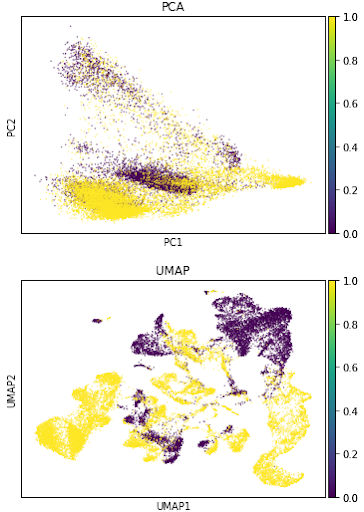
\includegraphics[width=0.5\textwidth]{disease_status.png}
  \caption{Principal Component and UMAP Projection visualizations colored by disease status. 0 is healthy, 1 is AA.}
  \label{PCA_projections_disease}
\end{figure}

\begin{figure}
  \centering
  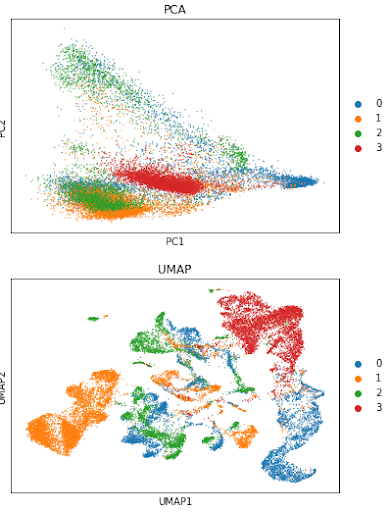
\includegraphics[width=0.5\textwidth]{individual.png}
  \caption{Principal Component and UMAP Projection visualizations colored by individual. Individuals 0 and 1 have AA. Individuals 2 and 3 are healthy controls.}
  \label{PCA_projections_individual}
\end{figure}


\section{Discussion and Results}

\subsection{Visualization reveals cells do not cluster by disease status}
Existing AA scRNA-seq data analysis uses linear dimensionality reduction techniques as a preprocessing step prior to clustering.
We began our analysis by following these same steps and assessing whether such preprocessing was sufficient for generating a dataset capable of training a simple but generalizable linear classifier.
We first visualized our data following a tutorial provided by the Scanpy[CITE] python package and qualitatively noticed that the diseased and healthy cells do not seem to cluster distinctly (see Figure \ref{PCA_projections_disease}).
We also noticed that cells from different individuals seemed to have very different transcriptional profiles (see Figure \ref{PCA_projections_individual}).
This led us to hypothesize that a linear model would either perform poorly when predicting disease status or perform well by learning to distinguish between individuals instead of distinguishing between disease status.

\subsection{LDA is insufficient for predicting disease status}
We performed five-fold cross validation on an LDA model trained on the first 50 principal components of the dataset and found the prediction accuracy to be an outlandishly high 98\%.
We subsequently hypothesised that this accuracy could be attributed to the model learning to distingish each individual as opposed to the model distinguishing between healthy and AA individuals.
To test this hypothesis, we used the same model hyperparameters but trained our model on data from exclusively one healthy and one AA individual.
Our hypothesis was that if the model is truly learning to distinguish between illness status, a model trained on data from representative AA patients and healthy individuals should be able to accurately predict the disease status of cells from other AA and healthy patients.
Conversely, if the model is learning to distingish individuals, a model trained on some individuals should not accurately predict the disease status of other individuals.
Because our dataset only contains data from four individuals, we trained the model on data from two individuals (one sick and one AA) and tested the model using the other two patients' data.
We then swapped the test and the training data and again assessed prediction accuracy.
Our measured prediction accuracy was 48.5\% and 67\%.
This decrease in accuracy supported our hypothesis that, even though it may be able to distinguish individuals, a simple linear model is not sufficient to reliably distinguish between AA and healthy cells.

We next considered whether larger principal components contained the dimensions along which the AA and healthy cells separated most distinctly and whether small variance introduced by the smaller principal components may be making the task of performing LDA more challenging.
To investigate this possibility, we ran this analysis again using only the first five principal components of the dataset.
This analysis yielded a prediction accuracies of 56.6\% and 60.4\%, leading us to conclude that even the largest principal components encompass variances unrelated to disease status.

\subsection{scVI does something I hope}
We discovered scVI through our class reading and wanted to investigate its performance on the \citet{tonglin_single-cell_2022} data.
We trained scVI on the \citet{tonglin_single-cell_2022} data using the scvi-tools python packge \citep{gayoso_python_2022} with the intention of exploring the differences in AA cell distributions vs healthy cell distributions in latent space.
We next wanted to build a simple classifier using this latent representation in order to create a path between the two cell-type distributions.
% - OR use pretrained scvi, transfer to AA data -- find bigger data of blood cells train SCVI, transfer to AA data real quick
% - OR use someone else's actual pretrained scvi
% 1. simple interpolation between samples from centroids of data domains
% 2. build simple classifier from latent representations -> use to create a path from sample to altered sample (like in original plan) 


\section{Conclusion}
scRNA-seq data is challenging to analyze due to the inherent noise, batch effects, dropout rates, and differences between individuals.
The challenge of accounting for person-to-person variability is amplified when there are a small number of individuals in your dataset.
The \citet{tonglin_single-cell_2022} data gave us an opportunity to experiment with a low-individual scRNA-seq dataset while working towards answering mechanistic questions about a devistating disease.
Our investigations revealed that simple linear models are insufficient for discriminating between disease states with such a low number of individuals.
Something about scVI.


{
\small
\printbibliography
}


\end{document}
